\chapter{Common Startup Mistakes}

This chapter follows the final practical movement of MIT OpenCourseWare's \emph{Nuts and Bolts of New Ventures}, curated by LazyingArt LLC through Video2Book. Marina Hatzopoulos is not giving a generic startup checklist. She is reconstructing, from the Z Corporation case, how a protected technical possibility becomes a product, a company, and a market. Bob frames the session as part of Joseph Hadzima's course: the speakers were not scripted, but the same themes kept recurring. We should therefore read the repetition as evidence from practice.

\section{A Deep-Tech Case Before the Rules}

Bob's handoff is important. Marina has noticed that some of her warnings overlap with earlier speakers. Bob tells the room that the course speakers did not coordinate their slides. If the same patterns recur, the repetition is not a slogan; it is convergence. That is the right frame for the chapter. We begin with a case, not a doctrine.

Marina begins with biography because it explains the mixture of skills the lecture will require. She studied math and music, then worked in banking, where she learned accounting, selling, and negotiation. At Thermo Electron, now Thermo Fisher, she discovered that evaluating a technology company was not just reading financial statements. It required judgment about the technology itself. That missing piece took her to MIT for a master's degree in mechanical engineering, not to become an engineer, but to manage engineers and speak their language.

The turning point was the Technology Licensing Office. MIT had patented inventions made by faculty and students, and the office looked for people and companies to commercialize them. There Marina encountered an early 3D-printing technology, before ``3D printing'' had become a common term. Professor Ely Sachs's group had been working on an ambitious printing project. Two engineers then turned the problem around: instead of designing a printhead around a chosen material system, they designed a material system around an off-the-shelf inkjet printhead. The first material story was deliberately crude: water, or ink, and cornstarch.

That reversal is already the deep-tech pattern. The company did not start with a finished product. It started with protected technical knowledge, a proof that the core science could work, and a large uncertainty about what market would care.

Z Corporation was founded in 1994 in Kendall Square. The company delivered its first product within about two years, reached profitability two years later, and eventually grew to
\begin{equation}
\text{revenue}\approx \$30\text{M},
\qquad
\text{employees}\approx 125.
\end{equation}
It did this with no venture capital. Marina is careful about that point: the absence of venture capital was not proof of superior wisdom. Nobody wanted to invest in a hardware business while the Internet market was taking off. The constraint nevertheless became part of the operating discipline.

The first time scale is therefore sober:
\begin{equation}
\text{deep-tech venture horizon}\sim 10\ \text{years}.
\end{equation}
For these notes, that is a boundary condition. Patents, proof of principle, market search, pricing, team formation, fundraising, and founder psychology all unfold inside a long hardware clock.

\section{Intellectual Property and Proof of Principle}

Marina next asks why someone creates a startup. The motive may be love of a technology, desire to solve a problem, independence, teamwork, community, or money. Her point is not moral ranking. The founder has to know the motive because the definition of success depends on it. A founder trying to improve brain-tumor diagnosis may make different choices from a founder whose primary aim is financial return.

Then the lecture narrows: when we are doing a deep-tech startup, the starting point should be intellectual property. A patent is presented as a bargain. We disclose how to do something, and in exchange receive a time-limited monopoly:
\begin{equation}
\text{patent protection}\approx 20\ \text{years}.
\end{equation}
This is not decorative law. In Z Corporation's case, Marina says a large customer took apart their machine, but did not launch a competing product until after the MIT patents expired. The patent period bought time to invest, educate the market, and grow.

The second rule concerns disclosure order:
\begin{equation}
\text{patent first}\quad\longrightarrow\quad \text{publish second}.
\end{equation}
The lecture states this as an operating rule for researchers and students. Publishing gives credibility, but premature publication can destroy patent protection. We do not need to expand this into a full legal doctrine here. The venture rule is enough: do not publish away the boundary that makes the technical advantage defensible.

The proof of principle is the next object. It is not the product. It is not even a usable prototype. It is the ugly machine that removes the central scientific doubt:
\begin{equation}
\text{proof of principle}
\neq
\text{finished product},
\qquad
\text{proof of principle}
\Rightarrow
\text{core technical risk reduced}.
\end{equation}
The early Z Corporation machine required manual powder handling and multiple computers. Its value was not elegance. It proved that a paper-printer-derived process could build a three-dimensional part.

\begin{remark}
For the rest of the lecture, intellectual property functions as a North Star. When the market is unclear, when customers disagree, and when the team is pulled in several directions, Marina returns to the same question: what makes us special that we can protect?
\end{remark}

\section{From Stealth to Market Disruption}

The first operational mistake is part-time entrepreneurship. Marina accepts Bob's earlier qualification: one should validate before quitting a job. But once the venture is validated and moving forward, time matters. A startup worked on for a few hours on Saturday morning will not move fast enough. Researchers need entrepreneurs, and entrepreneurs need researchers.

The next instinct is stealth. Founders fear that if they share the idea, someone will steal it. Marina's answer is practical: if all we have is an idea, then anyone can copy it once it reaches the market. The solution is not silence about the problem. The solution is patents, trade secrets, protected know-how, and disciplined judgment about what not to reveal. Customers do not need the inner workings. They need to know whether the product solves their problem.

The first market questions are therefore:
\begin{equation}
\text{painful problem?}
\qquad
\text{large enough market?}
\qquad
\text{worth entering?}
\end{equation}

\begin{figure}
\centering

\includegraphics[width=\linewidth]{lecture_10_figure_02.png}
\caption{Market disruption sources. The slide supplies the categories; the photograph is illustrative.}
\end{figure}

The slide gives a compact set:
\begin{equation}
D\in\{\text{regulations},\ \text{demographic changes},\ \text{new enabling technologies}\}.
\end{equation}
The transcript adds the important caveat. Some disruptions are too transient. Marina mentions corporate DEI spending and COVID-related startups as examples of openings that may not last long enough to support a durable company. Thus the test is not merely whether the world changed. It is whether the change persists long enough for company formation:
\begin{equation}
\text{startup opportunity}
\approx
\text{durable disruption}
+
\text{startup ability to move}.
\end{equation}

\subsection{Question \& Answer}

Why does disruption help a startup when large companies have almost every advantage?

Large companies have manufacturing, R\&D, sales, marketing, distribution, money, experience, brands, market knowledge, and customer relationships. Marina says they have nearly everything except the ability to pivot quickly. The startup edge is not that incumbents are stupid. The edge is maneuverability:
\begin{equation}
\text{startup edge}
=
\text{ability to pivot under incomplete information}.
\end{equation}
This matters because innovative markets do not present themselves as clean problem sets. We are not given all the variables. We are making decisions in fog. The startup must try, learn, and redirect.

\section{Market and Technology Development Interact}

The next movement is the lecture's main formal model. A deep-tech company develops two paths at once. One path is technical: run tests, try technology directions, isolate the highest-risk component, and de-risk it without building the whole system. The other path is market-facing: articulate what is special because of the IP, consider a wide range of industries, speak with experts, and test possible markets quickly.

The transcript gives a rough target for the early search:
\begin{equation}
N_{\text{market ideas}}\approx 20.
\end{equation}
This is not a statistical sample size. It is an antidote to premature narrowing. Marina calls the search speed dating, not dinner. We are looking for fast evidence, not perfect certainty.

\begin{figure}
\centering

\includegraphics[width=\linewidth]{lecture_10_figure_03.png}
\caption{Market and technology iteration. The slide's arrow is informal; it marks a practical feedback loop.}
\end{figure}

The visible slide notation is:
\begin{equation}
\text{iterative process}
\Rightarrow
\text{information from one drives the other}.
\end{equation}
For the notes, the cleaner reconstruction is:
\begin{equation}
\text{market learning}
\longleftrightarrow
\text{technology development}.
\end{equation}
The important constraint is that product-market fit cannot drift away from protectable differentiation. A market may be attractive, but if the company cannot protect the advantage there, the fit is strategically weak.

\begin{figure}
\centering
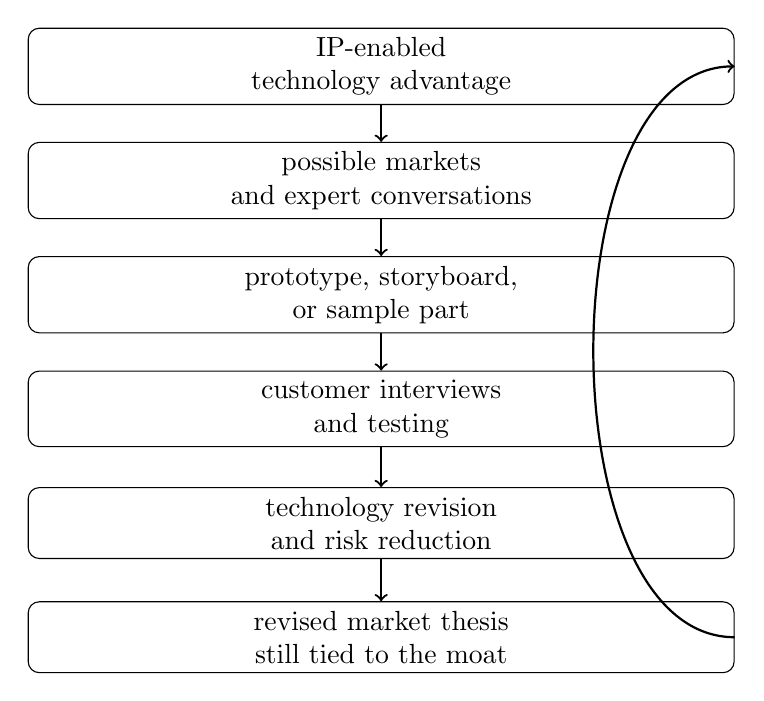
\begin{tikzpicture}[
  box/.style={draw, rounded corners, align=center, text width=0.72\linewidth, minimum height=0.88cm},
  arr/.style={->, thick}
]
\node[box] (ip) at (0,0) {IP-enabled\\technology advantage};
\node[box] (markets) at (0,-1.45) {possible markets\\and expert conversations};
\node[box] (proto) at (0,-2.90) {prototype, storyboard,\\or sample part};
\node[box] (test) at (0,-4.35) {customer interviews\\and testing};
\node[box] (revise) at (0,-5.80) {technology revision\\and risk reduction};
\node[box] (thesis) at (0,-7.25) {revised market thesis\\still tied to the moat};

\draw[arr] (ip) -- (markets);
\draw[arr] (markets) -- (proto);
\draw[arr] (proto) -- (test);
\draw[arr] (test) -- (revise);
\draw[arr] (revise) -- (thesis);
\draw[arr] (thesis.east) .. controls (2.1,-7.25) and (2.1,0) .. (ip.east);
\end{tikzpicture}
\caption{A pocket-safe reconstruction of the deep-tech feedback loop. The loop is narrow by design: the market and the technology revise one another, but the loop keeps returning to the moat.}
\end{figure}

\subsection{Question \& Answer}

How do we validate a deep-tech idea before there is a finished product?

Marina's answer is staged. First build the proof of principle to reduce the core technical risk. Then build a crude prototype, storyboard, or sample part. The artifact does not have to be beautiful. It has to be concrete enough that customers can react to something closer than an abstraction.

The update rule is:
\begin{equation}
\text{crude artifact}
\longrightarrow
\text{customer feedback}
\longrightarrow
\text{technical revision}
\longrightarrow
\text{better artifact}.
\end{equation}
In the Z Corporation story, Marina took sample parts to a trade show without even having a booth. Much of the feedback was negative: the parts were crude. But the conversation exposed the dimension that mattered. The parts were not perfect, but they could be made quickly.

The evidence hierarchy is:
\begin{align}
\text{compliment}
&< \text{reaction to idea} \\
&< \text{reaction to prototype} \\
&< \text{near-real product use} \\
&< \text{customer money}.
\end{align}
The closer the customer is to using the product as intended, the more useful the feedback becomes. Payment, deposits, and R\&D contracts are the strongest signals in the lecture.

\subsection{Question \& Answer}

What is deep tech in this lecture?

Marina defines it pragmatically. Deep tech is technology where the core science exists, often from university research, but the product will take a long time and substantial development to build:
\begin{equation}
\text{deep tech}
\approx
\text{core science exists}
+
\text{long development path}.
\end{equation}
Often it is a solution looking for a problem, not a problem already matched to a product. That is why the two paths must run in parallel. We do not know exactly where to take the technology until we learn who cares.

She is also careful about scope. When asked about software, AI, open-source models, and low-cost prototyping, she says that her experience is patentable hardware and that she is not the right person to answer the software/open-source version. These notes should preserve that boundary rather than inventing an IP framework she did not give.

\section{Differentiation, Customers, and the Pricing Pivot}

The lecture now shifts into its recurring rhythm: mistake, then instead. One mistake is to seek a popular market because everyone is talking about it. The founder imagines a crowded market must be promising, assumes incumbents are slow and stupid, and thinks the company can always lower price.

Marina rejects that logic. Lowering price is not the answer. In deep tech, the state of the art is the starting point, not the endpoint. The aim is to be better on a dimension the customer cares about and that the company can defend:
\begin{equation}
\text{protectable differentiation}
\Rightarrow
\text{possible premium price}.
\end{equation}

Competition is a double-edged sword. For Z Corporation, other 3D-printing firms helped educate the market. Once customers understood why they might need a 3D printer, Z Corporation could sell against alternatives by explaining that its machine was faster, cheaper, and capable of color. The worst competitor was often not another machine. It was doing nothing.

The central quantitative story begins with the initial market. High-end rapid-prototyping machines sold for roughly
\begin{equation}
\$100{,}000\ \text{to}\ >\$1{,}000{,}000.
\end{equation}
Z Corporation planned to enter at the low end with an office-compatible machine:
\begin{equation}
P_0=\$20{,}000.
\end{equation}
A year into development, before launch, two incumbents announced office-compatible machines at
\begin{equation}
P_{\text{incumbent}}=\$60{,}000.
\end{equation}
At the trade show, Z Corporation learned that its technology was approximately
\begin{equation}
\text{Z Corp speed advantage}\approx 10\times
\end{equation}
faster than the incumbent technologies. The surrounding transcript is partially garbled, but the repeated clear claim is speed. The parts had shortcomings, but customers cared that they could hold something quickly instead of waiting.

Walter Bornhorst, the chairman, proposed remaking the price decision:
\begin{equation}
\$20{,}000\longrightarrow \$60{,}000.
\end{equation}

\subsection{A Worked Decision Update}

We should write the pricing story as an update, not as a universal rule. Let \(P\) be the planned price and let \(E\) be the new evidence collected before launch:
\begin{equation}
E=
\{\text{incumbents at } \$60{,}000,\ 
\text{speed advantage}\approx 10\times,\ 
\text{customers care about speed}\}.
\end{equation}
The old plan was:
\begin{equation}
P_{\text{old}}=\$20{,}000.
\end{equation}
The revised decision was:
\begin{equation}
P_{\text{new}}
=
\mathrm{revise}(P_{\text{old}}\mid E)
=
\$60{,}000.
\end{equation}
The mathematical point is the conditional update:
\begin{equation}
\text{new strategic evidence}
\Rightarrow
\text{remake the strategic decision}.
\end{equation}
This does not mean ``triple the price.'' It means that price should track the value evidence, the competitive reference point, and the company's survival economics.

Marina adds a practical asymmetry:
\begin{equation}
\text{lowering price after launch is easier than raising price after launch}.
\end{equation}
The higher price mattered because production, sales, and market education were more expensive than expected. Educating the market took about:
\begin{equation}
\text{market-education cycle}\approx 1\ \text{year}.
\end{equation}

\subsection{Question \& Answer}

When should we listen to customers, and when should we ignore them?

Marina does not give a magic rule. Entrepreneurship constantly requires both listening and not listening. Customers may dismiss a new thing because they cannot yet imagine it. Industry veterans may reject anything unfamiliar. But feedback becomes stronger as it gets closer to real use:
\begin{equation}
\text{feedback value}
\uparrow
\quad\text{as}\quad
\text{use context approaches intended product use}.
\end{equation}

There is also danger on the opposite side. Power users can pull a company into a narrow, expensive direction. Z Corporation built a larger machine because many early customers asked for it. Later, Marina says the market was limited and the technical challenges were larger than expected. The project pulled against the long-term path of making machines less expensive and easier to use. The test is:
\begin{equation}
\text{customer request useful?}
\Longleftrightarrow
\text{request lies on the long-term strategic path}.
\end{equation}

This is why the North Star returns. If architecture customers cared about beautiful surface finish, but Z Corporation's protected advantage was speed, then architecture was not the right early market. The better question was: who cares about speed more than surface finish?

\section{Teams, Conflict, Priorities, and Cash}

The next mistakes are internal. Hiring people one trusts sounds reasonable, but loyal friends and family may not supply the missing skills. A famous board chair who is too busy may be less useful than a less famous person who is engaged. Z Corporation's founding team mattered because it combined business strategy, business execution, material science, software, and hardware.

The team rule is:
\begin{equation}
\text{founding strength}
\approx
\text{complementary skills}
+
\text{mutual respect}
+
\text{ability to make hard changes}.
\end{equation}
Marina adds a sharp practical warning: do not hire someone you cannot fire. If possible, work with someone before hiring. A one-week paid trial can reveal more than an interview.

The cultural mistake is to be merely nice. Marina distinguishes courtesy from avoidance. Z Corporation argued about everything, but without taking it personally and without grudges. That structure matters:
\begin{equation}
\text{diverse views}
+
\text{nonpersonal conflict}
\longrightarrow
\text{better decisions}.
\end{equation}
Negotiation is treated the same way: not a personality trait, but a skill to practice.

The next trap is confusing work volume with strategic work. A founder can get enormous satisfaction from checking off easy items. But the company needs the first item, not the seventeenth. Marina separates decisions:
\begin{align}
\text{strategic}
&=
\{\text{business},\ \text{team},\ \text{product},\ \text{pricing}\},\\
\text{non-strategic}
&=
\{\text{offices},\ \text{furniture},\ \text{software choice},\ \text{conference rooms}\}.
\end{align}
The strategic decisions must be remade when new information arrives:
\begin{equation}
\text{new information}
\Rightarrow
\text{remake strategic decisions}.
\end{equation}

No venture capital was not originally a chosen strategy for Z Corporation, but it shaped the company. Bootstrapping forced revenue, profitability, and cash discipline. Marina summarizes the case scale as:
\begin{equation}
\text{capital}\approx \$2.5\text{M},
\qquad
\text{revenue}\approx \$30\text{M},
\qquad
\text{employees}\approx 125.
\end{equation}
These are company facts, not a benchmark. The lesson is that financing constraints alter operating behavior.

This connects to two later mistakes. One is always staying positive: ignore bad news, believe the schedule, believe the cost estimate, and assume this time will be different. Marina's correction is to learn from failure and assume time and cost may be at least double what people say. Another is focusing only on growth. Growth matters, but companies die when they run out of cash:
\begin{equation}
\text{survival}
\Rightarrow
\text{track cash, time to revenue, and time to profitability}.
\end{equation}
A strong company may become an acquisition target. The immediate task is to build the strong company.

\section{Pitching, Funding, and the Venture-Capital Trap}

Investor communication is another place where founders put on a show. Marina warns against acronyms outsiders do not understand, complicated diagrams, tiny-font paragraphs, unrealistic projections, exit talk, confidentiality demands, and adding AI no matter what business one is in. The correction is simplification.

\begin{figure}
\centering

\includegraphics[width=\linewidth]{lecture_10_figure_04.png}
\caption{Simplifying the investor pitch. The slide contains the visible guideline of roughly 10--20 words per slide.}
\end{figure}

The visible presentation rule is:
\begin{equation}
\text{words per slide}\sim 10\text{--}20.
\end{equation}
The spoken pitch template is:
\begin{equation}
\text{We make \underline{\hspace{1.5cm}} for \underline{\hspace{1.5cm}} to \underline{\hspace{1.5cm}}.}
\end{equation}
The blanks are product, customer, and problem. If the listener cannot say what the product is, who the customer is, and what problem is being solved, technical detail will not rescue the pitch.

The funding map is broader than venture capital. Friends and family often come first. Angels can range roughly from:
\begin{equation}
\text{angel investment}\approx \$25{,}000\ \text{to}\ \$1{,}000{,}000.
\end{equation}
Government grants can be substantial in deep tech. Strategic investors may be suppliers, customers, or distributors. R\&D contracts are non-dilutive and validating. Customer deposits can also fund operations:
\begin{equation}
\text{customer deposit}=20\%,
\qquad
\text{delivery}\approx 3\text{--}6\ \text{months}.
\end{equation}
Venture capital and venture debt are part of the map, but they are not the universal destination.

\subsection{Question \& Answer}

Is venture capital always the right path?

No. Marina gives both sides. Venture capital can provide cash, advice, connections, and validation. Some companies need it. A two-sided global market, or a satellite company with high capital costs, may require large and fast financing.

But venture capital carries risks. Too much money can allow a company to move ahead before product-market fit is proven. Some markets cannot grow at the pace venture investors expect. Founders can lose control. High valuations raise the return bar. The more precise relation is:
\begin{equation}
\text{founder outcome}
\neq
\text{headline valuation}.
\end{equation}
A very profitable \(\$10\text{M}\) company that the founder owns entirely may be a better founder outcome than pushing for a billion-dollar business and failing. The correct financing path depends on the business.

Fundraising itself is work. Research investors before pitching them. If an investor funds only AI software and the company is selling 3D printers, do not pitch and call it optimism. Marina's rule is to reject yourself before collecting needless rejection. Every failed pitch should produce a strategic takeaway:
\begin{equation}
\text{failed pitch}
\longrightarrow
\{\text{wrong investor},\ \text{unclear pitch},\ \text{flawed business model}\}.
\end{equation}
Even rejection can be useful if it teaches whether the list, the communication, or the business model is wrong.

\section{CEO Syndrome and Course Closure}

The last founder mistake is psychological. Early CEOs are challenged constantly by engineers, customers, employees, and investors. That challenge forces rework: redesign the product, redefine product-market fit, and sharpen the value proposition. Then success arrives. People begin to call the CEO a visionary. Visibility and awards accumulate. New employees never saw the early uncertainty. The CEO starts to feel invincible.

The danger is a feedback loop in which success removes the challenge that produced success.

\begin{figure}
\centering
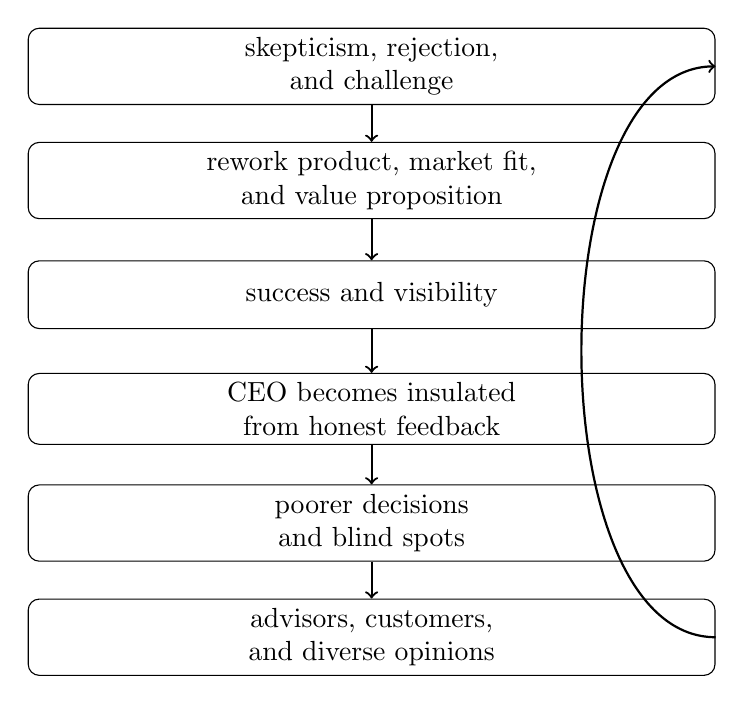
\begin{tikzpicture}[
  box/.style={draw, rounded corners, align=center, text width=0.70\linewidth, minimum height=0.86cm},
  arr/.style={->, thick}
]
\node[box] (challenge) at (0,0) {skepticism, rejection,\\and challenge};
\node[box] (rework) at (0,-1.45) {rework product, market fit,\\and value proposition};
\node[box] (success) at (0,-2.90) {success and visibility};
\node[box] (insulate) at (0,-4.35) {CEO becomes insulated\\from honest feedback};
\node[box] (bad) at (0,-5.80) {poorer decisions\\and blind spots};
\node[box] (advisors) at (0,-7.25) {advisors, customers,\\and diverse opinions};

\draw[arr] (challenge) -- (rework);
\draw[arr] (rework) -- (success);
\draw[arr] (success) -- (insulate);
\draw[arr] (insulate) -- (bad);
\draw[arr] (bad) -- (advisors);
\draw[arr] (advisors.east) .. controls (2.1,-7.25) and (2.1,0) .. (challenge.east);
\end{tikzpicture}
\caption{A conceptual reconstruction of CEO syndrome and its antidote. The challenge loop must be deliberately restored.}
\end{figure}

The antidote is not humility as decoration. It is structure: an advisory group willing to challenge ideas, customers close enough to the product to give real feedback, and a culture that asks questions and listens. Small rejections feel unpleasant, but they are the mechanism that improves decisions.

Marina closes her portion by restating the operating rules for deep-tech hardware: defensible product differentiation, a strong and diverse team, debate and healthy culture, customer contact, prototypes in customers' hands, revenue and profitability in the beachhead market, and decisions remade whenever new information arrives.

Bob then returns to the course as a whole. The course was not meant to be theory; it was meant to increase the probability of success. Entrepreneurship is a full-contact sport, not an academic exercise. The closing slide points students toward MIT's entrepreneurship resources.

\begin{figure}
\centering

\includegraphics[width=\linewidth]{lecture_10_figure_05.png}
\caption{MIT entrepreneurship roadmap. The detailed logos are best preserved as screenshot evidence rather than redrawn.}
\end{figure}

The visible roadmap includes participation counts:
\begin{equation}
50{,}000+,\quad 5{,}000+,\quad 2{,}000+,\quad 350,\quad 72.
\end{equation}
The small labels are dense, so the notes should preserve the screenshot and summarize the large movement: inspiration, exploration, fundamentals, application, and acceleration. Bob also names the Venture Mentoring Service as a resource where entrepreneurs receive homework, mentor teams, and regular meetings.

The final formula is Joseph Hadzima's course heuristic:
\begin{equation}
H=\frac{R}{E}.
\end{equation}
Here \(H\) is happiness, \(R\) is reality, and \(E\) is expectations. Bob's interpretation is practical: ask whether we can create a reality that exceeds the expectations people have. The same fraction applies to customers, investors, employees, and founders themselves.

\section{Summary}

The lecture begins with a case and ends with a course-wide rule. In between, the argument is consistent. Deep-tech entrepreneurship starts with protected differentiation, then tests market reality without giving away the core secret. We should expect fog, incomplete information, and wrong turns. The work is to build enough proof to learn, enough customer contact to steer, enough team conflict to decide well, and enough financial discipline to survive.

The central update is the Z Corporation pricing decision:
\begin{equation}
(\$20{,}000,\ \text{low-end entry})
\quad
\stackrel{\text{new evidence}}{\longrightarrow}
\quad
(\$60{,}000,\ \text{premium speed value}).
\end{equation}
That is the lecture in miniature. A startup is not a fixed plan. It is a protected technical possibility learning its way through the market.